\chapter{DSDV}
\label{chap:dsdv}

\section{Ejercicio 2.1}

\subsection{Avanza la simulación hasta el instante t = 7 s. Busca el primer paquete Hello transmitido a partir a ese
instante con un valor de hopdistance de al menos 3 y muestra una captura del contenido. Explica el significado
de los campos srcAddress y nextAddress, utilizando para explicarlos una captura de la tabla de enrutamiento del
nodo que está transmitiendo el paquete (i.e., no el que consta en srcAddress)}

\begin{figure}[H]
    \centering
    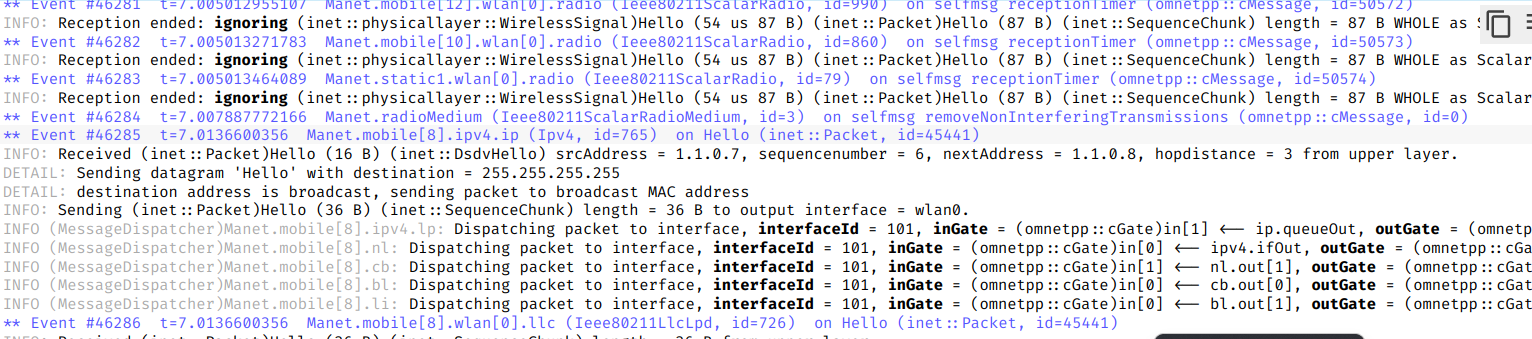
\includegraphics[width=155mm, scale=0.75]{imaxes/dsdv/ejercicio2_1.png}
    \caption{Log del nodo que manda el primer Hello con hopdistance 3}
    \label{fig:ejer2_1}
\end{figure}

Como se puede ver la imagen, el nodo que manda el primer mensaje Hello con hopdistance 3 es el nodo 8. Vamos a fijarnos en su tabla de enrutamiento:

\begin{figure}[H]
    \centering
    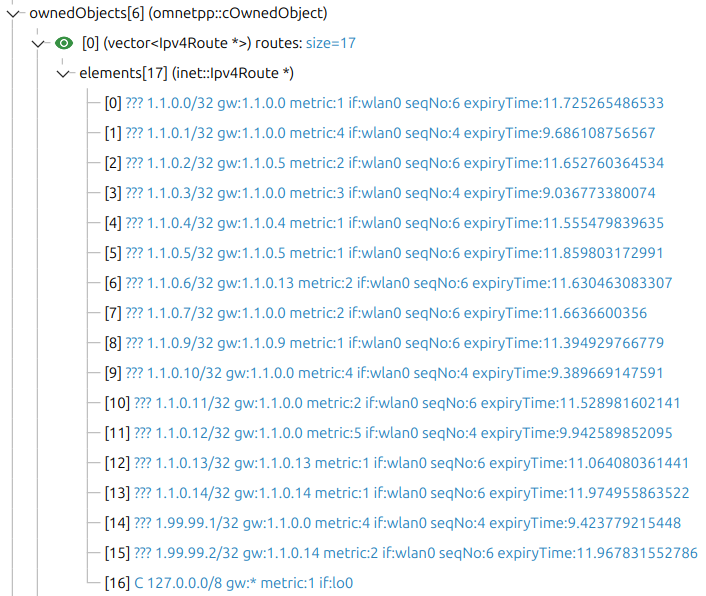
\includegraphics[width=115mm, scale=0.75]{imaxes/dsdv/ejercicio2_1_2.png}
    \caption{Tabla de enrutamiento nodo 8}
    \label{fig:ejer2_1_2}
\end{figure}

Los mensajes Hello contienen las entradas de la tabla de enrutamiento de ese nodo. En Inet no se manda toda las entradas de la tabla en un mensaje Hello, si no que manda una o algunas veces varias entradas. Según la imagen \ref{fig:ejer2_1}, el campo srcAddress es el nodo que generó el paquete Hello, en este caso es el 1.1.0.7. El campo nextAddress es la siguiente dirección que va a retransmitir el Hello, en este caso 1.1.0.8. Como 1.1.0.8 (nodo 8) tiene en su tabla de enrutamiento una métrica de 2 para 1.1.0.7 (nodo 7) (imagen \ref{fig:ejer2_1_2}), va a sumar 1 para transmitir el Hello a los vecinos indicando que el nodo destino está a 3 saltos del nodo 7.



\section{Ejercicio 2.2}

\subsection{¿Qué valor tiene de sequencenumber? ¿Qué quiere decir ese valor?}

Como se puede ver en la imagen \ref{fig:ejer2_1}, el campo sequencenumber tiene valor 6. Este valor ayuda a identificar entradas obsoletas o inválidas (un nodo se ha desplazado y ya no es alcanzable) con el fin de evitar bucles. Para ver si una ruta es válida o inválida llega con ver si este valor es par (ruta disponible) o impar (ruta no disponible/caída). De esta forma, nos indica como de actualizado está la información de la ruta, el estado de la ruta y evitar posibles conflictos en la red.

\section{Ejercicio 2.3}

\subsection{¿Cómo se modifica? ¿Qué nodo lo modifica, y cuándo lo hace?}

Este valor lo modifica el propio nodo en su tabla de enrutamiento, incrementándolo en 2 cuando la ruta que es válida, pero si un nodo identifica un nodo caído (o que se desplazó), el nodo que identifica la caída puede cambiar en la entrada de la tabla, el valor del sequencenumber de otro nodo indicando que es inválido. Esto se indica incrementando el valor 1 número (las rutas válidas tienen valor par, si incrementamos a 1, pasa a ser impar y por lo tanto indicando que ya no es un nodo válido). 

Cuando un nodo descubre una ruta mejor hacia el destino, actualiza este valor. Esto ocurre si el nuevo número de secuencia recibido es mayor (y par), con respeto a lo que tiene el guardado en su tabla de enrutamiento, por lo registra en su tabla y actualiza el nodo que recibió la información (en este caso mobile[8]). En el caso de una ruta no válida, genera un sequencenumber impar y establece el costo de la ruta como infinito para indicar que esa ruta no se puede usar.

El caso de una ruta inválida, es el otro nodo el que lo actualiza. Esto ocurre básicamente porque en el caso de que el nodo que identifica otro nodo inválido se moviera y un nodo en su tabla de enrutamiento tuviera registrado el nodo inválido con un sequencenumber impar, este al ver que si que es alcanzable, como el nodo inválido tiene un sequencenumber mayor, el otro nodo puede actualizarlo ya como valido y no pasaría nada.

\section{Ejercicio 2.4}

\subsection{Muestra la tabla de enrutamiento del nodo que recibe el Hello de la pregunta anterior justo antes y justo
después de recibirlo, relacionándola con el contenido del paquete. Si se actualiza la tabla, explica por qué se
actualiza y las entradas que se crean. Si no se actualiza, explica por qué no se actualiza y di qué entrada se
crearía (destino, gateway, métrica) si se actualizase con la información del paquete.}

\begin{figure}[H]
    \centering
    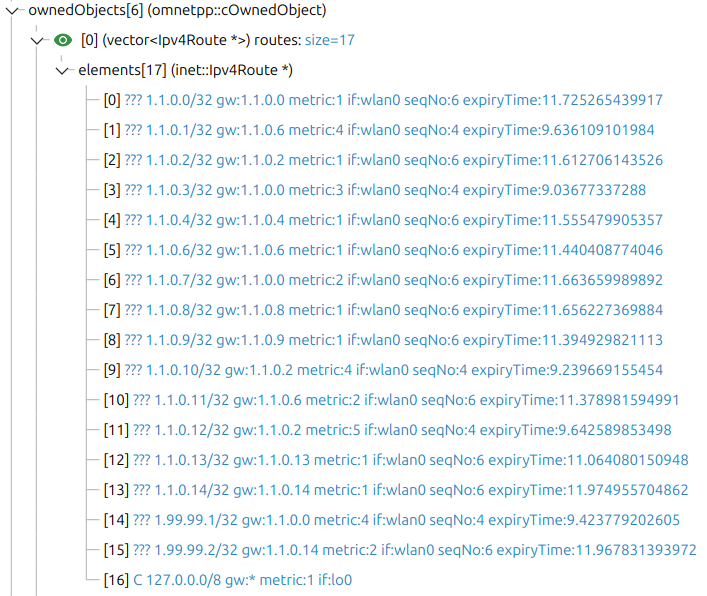
\includegraphics[width=115mm, scale=0.75]{imaxes/dsdv/ejercicio2_4_nodo5.png}
    \caption{Tabla de enrutamiento nodo 5 antes recibir Hello de nodo 8}
    \label{fig:ejer2_4_1}
\end{figure}

\begin{figure}[H]
    \centering
    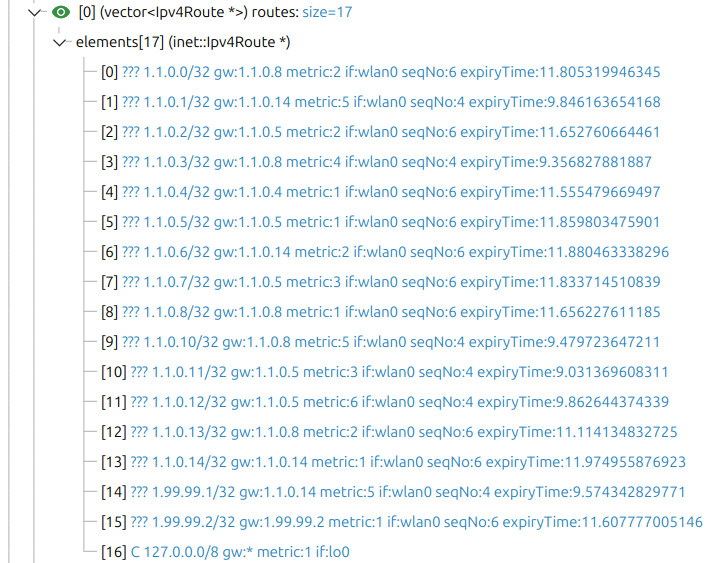
\includegraphics[width=115mm, scale=0.75]{imaxes/dsdv/ejercicio2_4_nodo9.png}
    \caption{Tabla de enrutamiento nodo 9 antes recibir Hello de nodo 8}
    \label{fig:ejer2_4_2}
\end{figure}

En las anteriores imágenes (\ref{fig:ejer2_4_1} y \ref{fig:ejer2_4_2}) podemos ver las tablas de enrutamiento antes de recibir el Hello, de los nodos 5 y 9, que son nodos que está dentro del rango del nodo 8. Ambas tienen para la entrada al nodo 7 un numero de secuencia 6. En el nodo 5 tiene una métrica de 2 y el gateway es el nodo 0, mientras que el nodo 9 tiene una métrica de 3 y el gateway es el nodo 5. 

En las siguientes imágenes vamos a ver las tablas de enrutamiento de los dos nodos mencionados anteriormente, pero después de haber recibido el mensaje Hello:

\begin{figure}[H]
    \centering
    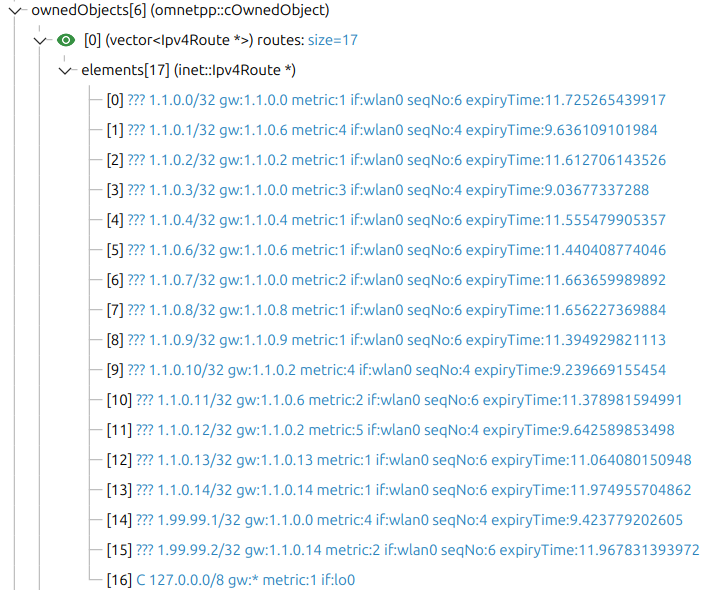
\includegraphics[width=115mm, scale=0.75]{imaxes/dsdv/ejercicio2_4_1_nodo5.png}
    \caption{Tabla de enrutamiento nodo 5 antes recibir Hello de nodo 8}
    \label{fig:ejer2_4_3}
\end{figure}

\begin{figure}[H]
    \centering
    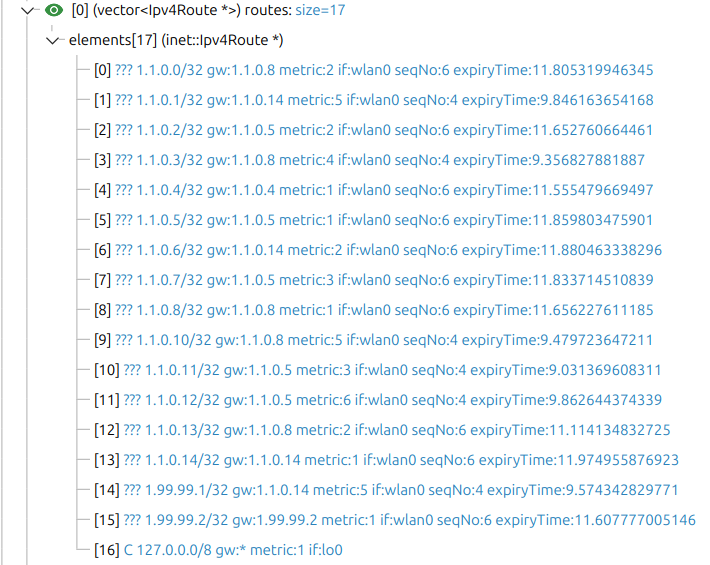
\includegraphics[width=115mm, scale=0.75]{imaxes/dsdv/ejercicio2_4_1_nodo9.png}
    \caption{Tabla de enrutamiento nodo 9 antes recibir Hello de nodo 8}
    \label{fig:ejer2_4_4}
\end{figure}


Como podemos ver, ninguna de las tablas de enrutamiento han cambiado. Esto pasó ya que el mensaje Hello que ha mandado el nodo 8, manda una entrada de su tabla de enrutamiento con un sequencenumber igual al que tienen los otros nodos en su tabla de enrutamiento, por lo que no se actualiza nada.

Como se ve en la figura \ref{fig:ejer2_1_2}, la entrada que tiene el nodo 8 para el nodo 7 es el mismo gateway que tiene el nodo 5 y 9. En el caso de la métrica, como el nodo 5 tiene hopdistance mayor o igual al que guarda (marca hopdistance 3 y en el nodo 5 y 9 tiene una métrica de 2 y 3 respectivamente), tampoco lo actualizan. 

En el caso de que recibieran un sequencenumber mayor y par, no se crearía ninguna entrada, solamente se actualizaría cambiando la métrica. Para el caso del hopdistance, si los nodos 5 y 9 guardasen un número mayor que el que recibieran, significaría que el nodo 8 estaría más cerca por lo que se actualizaría el valor. El gateway en el caso de que se actualizase la entrada de alguno de los nodos, el gateway pasaría a ser el del nodo 8.

En el caso de que recibiera un sequencenumber mayor y impar, tampoco se crearía ninguna nueva entrada, solamente se actualizaría ese valor para saber que el nodo es inalcanzable, aunque en el caso de que otro nodo ajeno le mandara un Hello con la entrada de ese nodo válido, lo volvería a actualizar.


\section{Ejercicio 2.5}

\subsection{Avanza hasta la caída del nodo en t = 15 s. Ten en cuenta que la ruta en ese momento puede ser diferente a
la de AODV, y por lo tanto el nodo a desactivar también. ¿Cuál es el primer nodo en darse cuenta de la caída?
¿Notifica la caída del nodo de alguna forma?}

Hay que aclarar que hemos cambiado de semilla ya que con DSDV no funcionaba bien con la semilla que usamos en los anteriores apartados. La semilla a utilizar en este apartado y para el siguiente es 1865.

Ruta antes de la caída:

\begin{figure}[H]
    \centering
    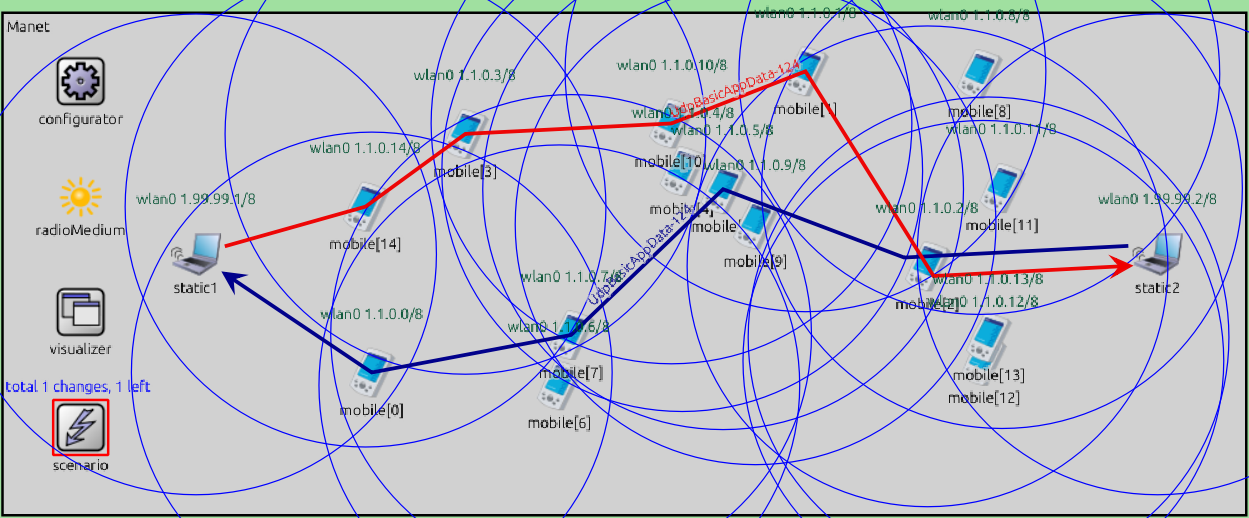
\includegraphics[width=115mm, scale=0.75]{imaxes/dsdv/ejercicio2_5.png}
    \caption{Ruta antes de la caída}
    \label{fig:ejer2_5_1}
\end{figure}


Como nodo 2 es el nodo más próximo a static2 que establece la ruta, vamos a provocar su caída. Cuando el nodo está caído, vemos que el nodo 1, que es el nodo que está en la ruta y alcanza a nodo 2 manda varios UDP datas hasta que llega al límite (solo envía 6 veces, a la séptima para). Esto se puede ver en la siguiente imagen:

\begin{figure}[H]
    \centering
    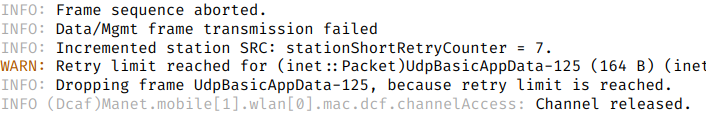
\includegraphics[width=115mm, scale=0.75]{imaxes/dsdv/ejercicio2_5_1.png}
    \caption{Mensaje del nodo 1 cuando no es capaz de enviar los UDP datas al detectar un nodo caído}
    \label{fig:ejer2_5_2}
\end{figure}


Esto quiere decir que el nodo 1 es el primero en ver que el nodo 2 está caído, ya que no puede procesar los paquetes UDP. El problema es que INET no tiene forma de notificar la caída, es decir, en las tablas de enrutamiento no cambia el sequencenumber a un número impar para indicar qué nodo ya no es válido, por lo que no hay forma de notificar eso de una forma eficaz.



\section{Ejercicio 2.6}

\subsection{¿Cómo se repara la ruta entre static1 y static2? ¿En qué momento?}

La ruta de static1 a static2 se repara cuando todos los nodos mandan sus mensajes Hello actualizando la tabla de enrutamiento y todo el mundo conoce el cambio de topología que hay en la red gracias a los mensajes UDP Data. Es decir, cuando las tablas de enrutamiento y topología de la red están actualizadas, los nodos crean una ruta. La nueva ruta se puede ver en la siguiente imagen:

\begin{figure}[H]
    \centering
    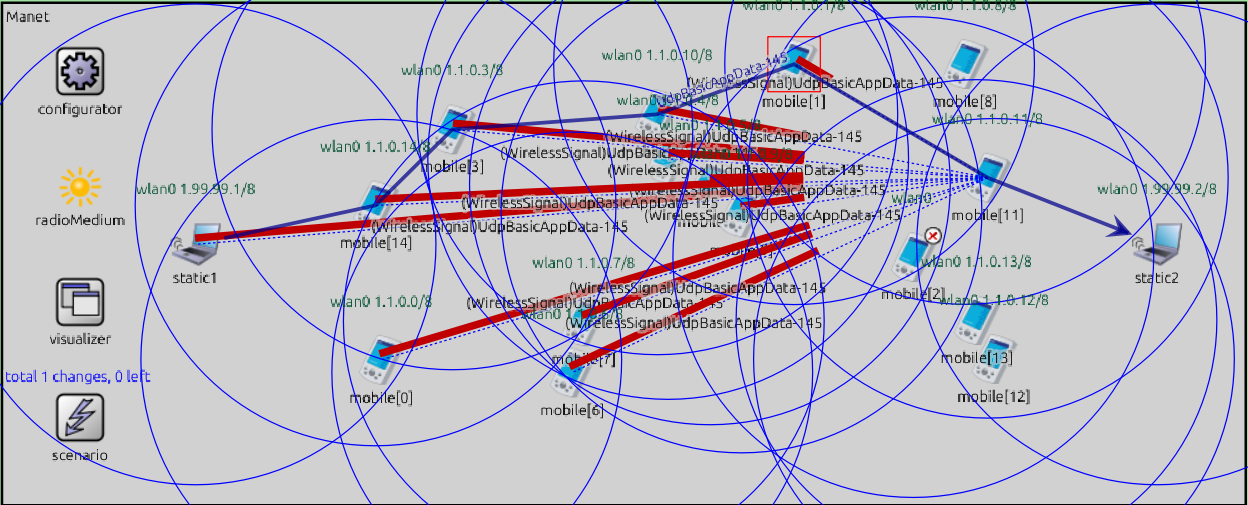
\includegraphics[width=115mm, scale=0.75]{imaxes/dsdv/ejercicio2_6.png}
    \caption{Ruta nueva después de la caída del nodo 2}
    \label{fig:ejer2_6}
\end{figure}

Por ejemplo, antes de establecer la nueva ruta, si vemos la tabla de enrutamiento de un nodo antes de que static2 enviara un Hello y después de recibir ese Hello, vemos que ha cambiado:

\begin{figure}[H]
    \centering
    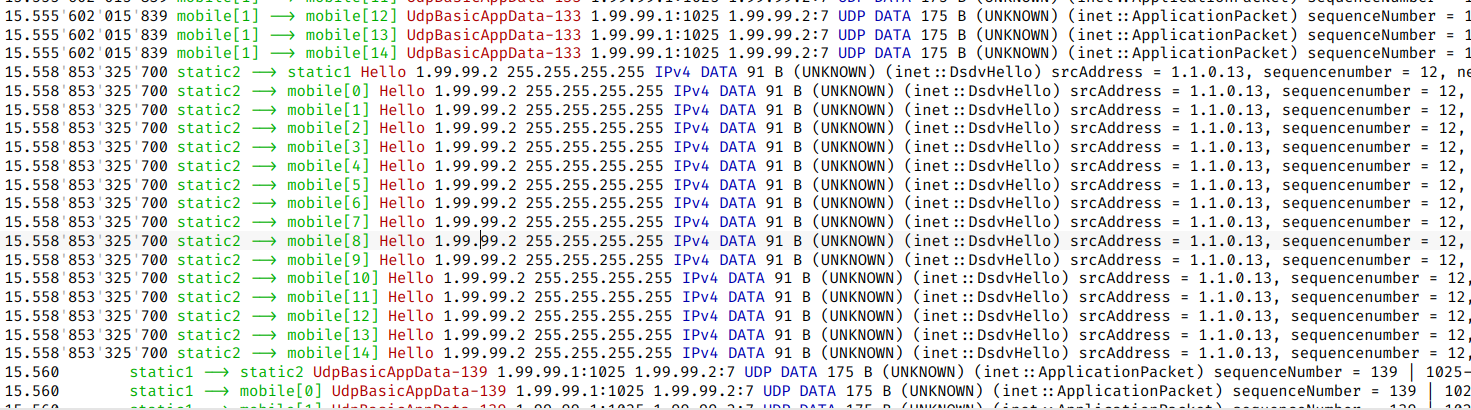
\includegraphics[width=145mm, scale=0.75]{imaxes/dsdv/ejercicio2_6_1.png}
    \caption{Stati2 mandando mensaje Hello}
    \label{fig:ejer2_6_1}
\end{figure}

\begin{figure}[H]
    \centering
    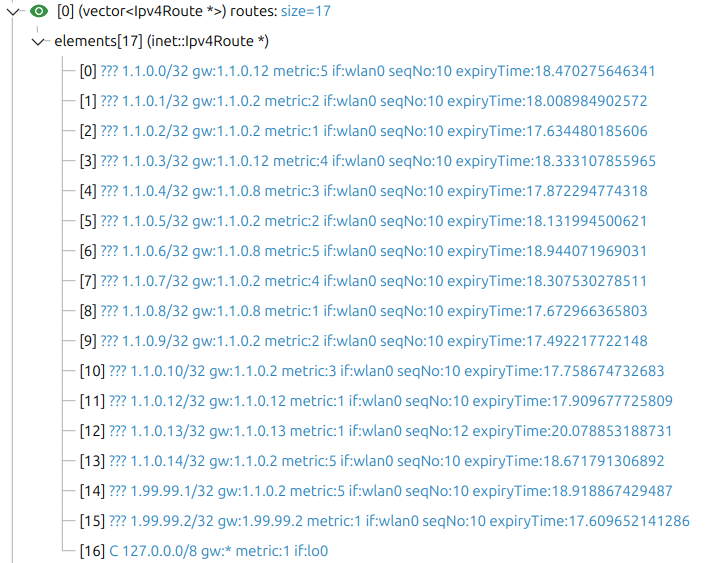
\includegraphics[width=115mm, scale=0.75]{imaxes/dsdv/ejercicio2_6_2.png}
    \caption{Nodo 11 antes de recibir Hello de static2}
    \label{fig:ejer2_6_2}
\end{figure}

\begin{figure}[H]
    \centering
    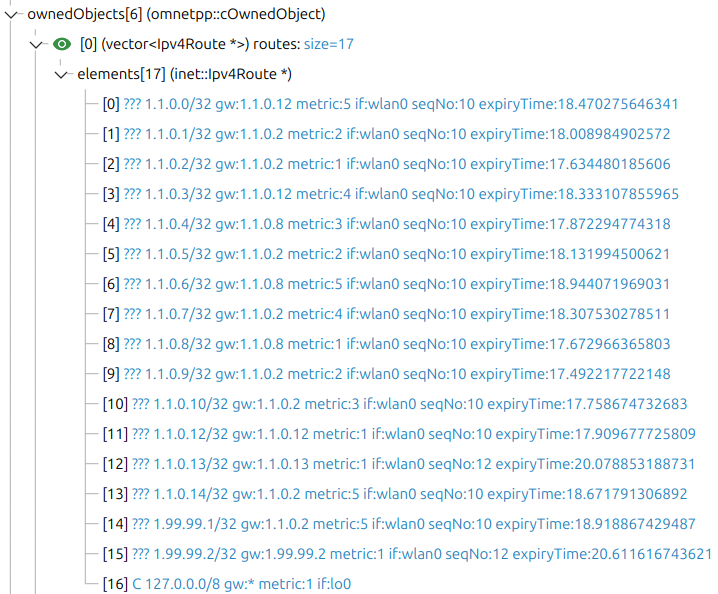
\includegraphics[width=115mm, scale=0.75]{imaxes/dsdv/ejercicio2_6_3.png}
    \caption{Nodo 11 después de recibir Hello de static2}
    \label{fig:ejer2_6_3}
\end{figure}

Si comparamos la imagen \ref{fig:ejer2_6_2} con \ref{fig:ejer2_6_3} la entrada de static2 en el nodo 11 ha cambiado. Este paso se repite para todos los demás nodos y, una vez tienen la tabla de enrutamiento actualizada, se establecería la ruta que aparece en la imagen \ref{fig:ejer2_6}

